\chapter{Figures and tables}

\section{Figures}
All figures should be positioned at a good position near to corresponding text. The \verb|figure| environment must be used to create figures. You are highly encouraged to create publication quality \emph{vector} pictures. Here is an example of creating a figure and then referring to it.

Figure~\ref{fig:CoverPic} illustrates the development of streamwise velocity in the planar asymmetric diffuser. In this figure, the numerical results are validated with the experimental data. An example of \verb|subfigure| environment is also shown in Figure~\ref{fig:Cf}.
 
\begin{figure}[!htbp]
	\centering
	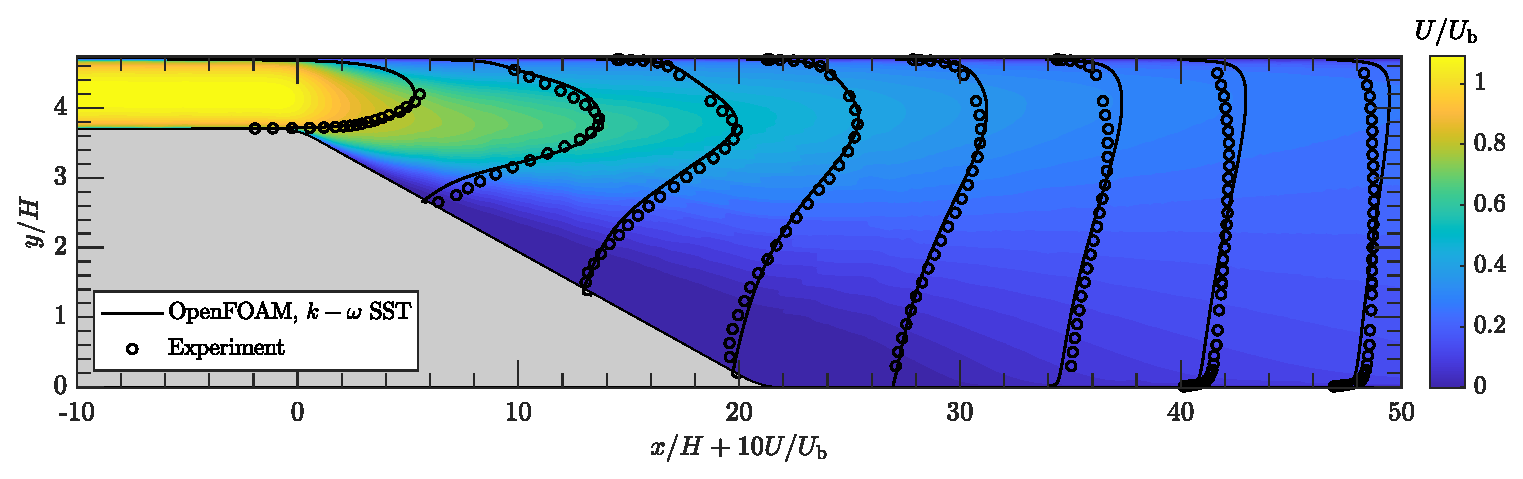
\includegraphics[width=1\textwidth]{Figures/CoverPic}
	\caption{Development of streamwise velocity in the planar asymmetric diffuser}
	\label{fig:CoverPic}
\end{figure} 



\begin{figure}[!hbpt]
	\centering
	\begin{subfigure}[t]{0.48\textwidth}
		\centering
		\includegraphics[width=1\textwidth]{Figures/cf_lowerWall}
		\caption{Lower wall}
		\label{fig:Cf_L}
	\end{subfigure}
	\hspace{0.02\textwidth}
	\begin{subfigure}[t]{0.48\textwidth}
		\centering
		\includegraphics[width=1\textwidth]{Figures/cf_upperWall}
		\caption{Upper wall}
		\label{fig:Cf_U}
	\end{subfigure}
	\caption{Skin friction coefficient on both walls}
	\label{fig:Cf}
\end{figure}



\section{Tables}

A table example is shown in Table~\ref{tab:exampleTable}. You can use online latex table generator tools to produce more advanced tables (e.g. \href{https://www.tablesgenerator.com/}{www.tablesgenerator.com}).


\begin{table}[t]
	\caption{Table caption}
	\label{tab:exampleTable}
    \centering
	\begin{tabular}{l l l}
		\hline
		Example & Time & Cost \\
		\hline
		1 & 12.5 & \$1,000 \\
		2 & 24 & \$2,000 \\
		3 & 36 & \$4,000 \\
		4 & 48 & \$8,000 \\
		\hline
	\end{tabular}
\end{table}